\subsection{Mobile robot}
\label{sec:mobile}

Mobile robots (or telerobot) have the capability to move around
in their environment and are not fixed to one physical location.
\\
As stated in \cite{robot:whereami}, Leonard and Durrant-Whyte
(in 1991) summarized the general problem of mobile robot navigation
by three questions:

\begin{itemize}
\item \texttt{Where am I ?}
\item \texttt{Where am I going ?}
\item \texttt{How should I get there ?}
\end{itemize}

This section surveys the some basic notitions in sensors 
and technologies that aim at answering the
first question.
\\
We will often refer to the expression \textit{robot navigation},
that is primarily about guiding a mobile robot to a desired destination
or along a pre-specified path. For these reasons teleoperator must
be able, with an as great as possibile precision, to know the robot's
position in its environment, which consists of landmarks and obstacles.
\\
In order to achieve this objective the robot needs to be equipped with
sensors suitable to localise the robot throughout the path it is to follow.
These sensors may give overlapping or complementary information and may
also sometimes be redundant. Because of the lack of a single, generally
good method, developers of  automated guided vehicles (AGVs) and mobile
robots usually combine two or more methods to localize the robot.
\\
All these sensor measurements can be fused to estimate the robot's
position by using a sensor fusion algorithm. Sensor fusion
in this case is the method of integrating data from distinctly
different sensors to estimate the robot's position.
\\
The sensors used to localize the mobile robot can be categorized into
two groups: internal and external sensors. The ones belowing to the first
group measure some internal state of the robot, such as motion, acceleration,
direction.
\\
Sensors belowing to the second group (external sensors) provide information
about objects in the workspace surrounding the robot.
\\
Sensors that will be exposed in this section are:
\begin{itemize}
\item \texttt{Optical Encoder} \\
  Interanl sensor, details in chapter \ref{sec:mobile:encoder}
\item \texttt{Laser} \\
  External sensor, details in chapter \ref{sec:mobile:laser}
\item \texttt{Sonar} \\
  External sensor, details in chapter \ref{sec:mobile:sonar}
\item \texttt{Bumper} \\
  External sensor, details in chapter \ref{sec:mobile:bumper}
\item \texttt{Vision} \\
  External sensor, details in chapter \ref{sec:mobile:vision}
\end{itemize}

Data collected with previous sensors must be processed with proper methods to
determinate robot's position. Among these we will briefly cite: 
\begin{itemize}
\item \texttt{Odometry} \\
  Details in chapter \ref{sec:mobile:odometry}
\item \texttt{Inertial Navigation} \\
  Details in chapter \ref{sec:mobile:inertial}
\item \texttt{Magnetic compass} \\
  Details in chapter \ref{sec:mobile:compass}

\item \texttt{Video based positionig} \\
  Details in chapter \ref{sec:mobile:video}
\end{itemize}

%%------------------------------------------------------------------

\subsubsection{Optical Encoder}
\label{sec:mobile:encoder}


The simplest type of incremental encoder is a single-channel
\textit{tachometer encoder}, basically an instrumented mechanical
light chopper that produces a certain number of sine or square wave
pulses for each shaft revolution. Adding pulses increases the resolution
(and subsequently the cost) of the unit.
\begin{figure} [h]
  \begin{center}
    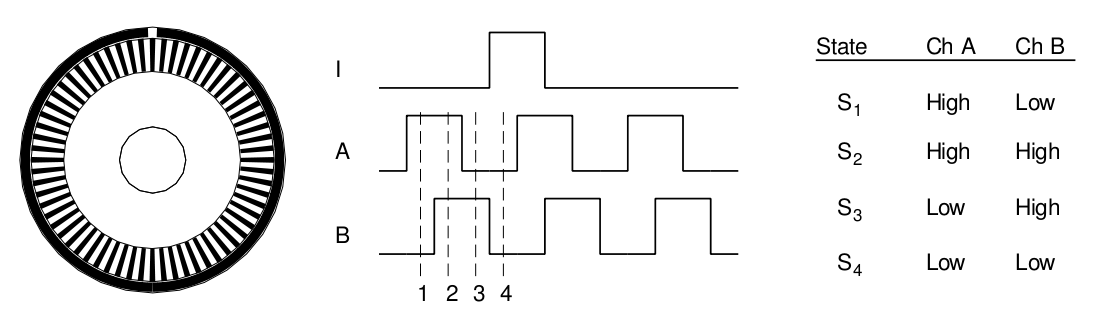
\includegraphics[width=\textwidth]{img/incremental_encoder.png}
    \caption{The observed phase relationship between Channel A and B
      pulse trains can be used to determine
      the direction of rotation with a phase-quadrature encoder,
      while unique output states S1 - S4 allow for up to a
      four-fold increase in resolution. The single slot in the outer
      track generates one index pulse per disk rotation.
    }
    \label{fig:incremental_encoder}
  \end{center}
\end{figure}
These relatively inexpensive devices are well suited as velocity feedback
sensors in medium to high speed control systems, but run into noise and
stability problems at extremely slow velocities due to quantization errors.
\\
The tradeoff here is resolution versus update rate: improved transient
response requires a faster update rate, which for a given line count reduces
the number of possible encoder pulses per sampling interval. 
\\
In addition to low-speed instabilities, single-channel tachometer encoders
are also incapable of detecting the direction of rotation and thus cannot
be used as position sensors. Phase-quadrature incremental encoders overcome
these problems by adding a second channel, displaced from the
first, so the resulting pulse trains are 90 degrees out of phase, as shown
in figure \ref{fig:incremental_encoder}.
\\
This technique allows the decoding electronics to determine which channel
is leading the other and hence ascertain the direction of rotation, with the
added benefit of increased resolution.
\\
The incremental nature of the phase-quadrature output signals dictates that
any resolution of angular position can only be relative to some specific
reference, as opposed to absolute. Establishing such a reference can be
accomplished in a number of ways. For applications involving continuous
360-degree rotation, most encoders incorporate as a third channel a special
index output that goes high once for each complete revolution of the shaft
(see figure \ref{fig:incremental_encoder}).
\\
Intermediate shaft positions are then specified by the number of encoder
up counts or down counts from this known index position.
\\
One disadvantage of this approach is that all relative position information
is lost in the event of a power interruption.
\\
Interfacing an incremental encoder to a computer is not a trivial task.
A simple state-based interface as implied in Figure 1.1 is inaccurate if
the encoder changes direction at certain positions, and false pulses can
result from the interpretation of the sequence of state changes.
\\
Absolute encoders are typically used for slower rotational applications
that require positional information when potential loss of reference
from power interruption cannot be tolerated.
\\
Instead of the serial bit streams of incremental designs, absolute optical
encoders provide a parallel word output with a unique code pattern for each
quantized shaft position. The most common coding schemes are \textit{Gray code},
natural binary, and binary-coded decimal.
\\
The Gray code (for inventor Frank Gray of Bell Labs) is characterized by the
fact that only one bit changes at a time, a decided advantage in eliminating
asynchronous ambiguities caused by electronic and mechanical component tolerances
(see figure \ref{fig:absolute_encoder} a).
\begin{figure} [h]
  \begin{center}
    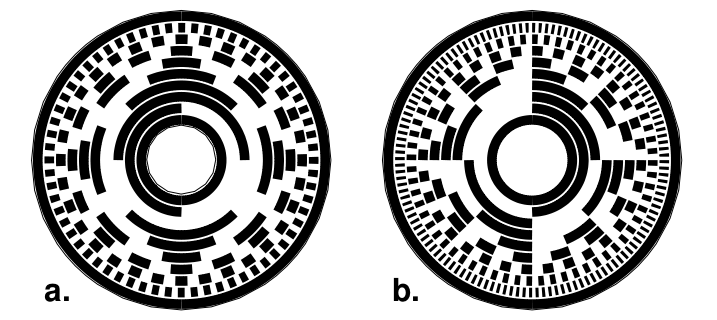
\includegraphics[width=300pt]{img/absolute_encoder.png}
    \caption{Rotating an 8-bit absolute Gray code disk.
      a. Counterclockwise rotation by one position increment will cause
      only one bit to change.
      b. The same rotation of a binary-coded disk will cause all bits to
      change in the particular case (255 to 0) illustrated by the
      reference line at 12 o'clock.}
    \label{fig:absolute_encoder}
  \end{center}
\end{figure}
Binary code, on the other hand, routinely involves multiple bit changes when
incrementing or decrementing the count by one. For example, when going from
position 255 to position 0 in figure \ref{fig:absolute_encoder} b, eight
bits toggle from 1s to 0s. Since
there is no guarantee all threshold detectors monitoring the detector elements
tracking each bit will toggle at the same precise instant, considerable ambiguity
can exist during state transition with a coding scheme of this form.
\\
Some type of handshake line signaling valid data available would be required
if more than one bit were allowed to change between consecutive encoder positions.
\\
Absolute encoders are best suited for slow and/or infrequent rotations such
as steering angle encoding, as opposed to measuring high-speed continuous
(i.e., drive wheel) rotations as would be required for calculating displacement
along the path of travel.
\\
A potential disadvantage of absolute encoders is their parallel data output,
which requires a more complex interface due to the large number of electrical leads.


\subsubsection{Laser}
\label{sec:mobile:laser}

The Laser sensor is used to measure distance.
\\
The sensor, by a mechanical mechanism with a mirror, sweeps
transmitted and received beams coaxial.
\\
% Figure 2.4: Laser sensor with rotating mirror

The transmitter illuminates a target with a collimated beam
and it received the reflected beam detects the time needed for
round-trip. The distance to an object can be achieved by measuring
the time of flight or the phase shift.
\\
The time of flight is the time between transmission and reception
of the light pulse. This time is directly proportional to the distance
between the scanner and the object.
\\
If you indicate with \textit{L} the distance between the laser and
the obstacle and with \textit{c} the light speed, the proper formula
to retrieve time of fligh is:

\[
t_{flight} = \frac{2L}{c}
\]

so

\[
L = \frac{t_{flight}}{2}c
\]


  
\begin{comment}                          
The quality of time of flight range sensors manly depends on:
         • Uncertainties about the exact time of arrival of the reflected signal
         • Inaccuracies in the time of fight measure
         • Interaction with the target (surface, specular reflections)
         • Variation of propagation speed
         • Speed of mobile robot and target (if not at stand still).
The Phase-Shift measurement produces a range estimation.
We can indicate with:
 f the modulating frequency,
c the light speed,
          c
 λ=          ,
          f
D′ is the distance covered by the emitted light
                                                            θ
                                      D′ = L + 2D = L +         λ
                                                          2 ⋅π
D distance between the beam splitter and the target
                                                    λ
                                                       θ
                                             D=
                                                  4 ⋅π
where θ is the phase difference between the transmitted and the reflected beam.
                          Figure 2.5: Transmitted and Reflected beam
                                                                                        20
                                                                             Chapter 1
Confidence in the range (phase estimate) is inversely proportion to the square of the
received signal amplitude.
In the Figure 2.5 is possible see a typical range image of a 2D laser range sensor with
a rotating mirror. The lengths of the lines through the measurement points indicate
the uncertainties.

\end{comment}

\subsubsection{Sonar}
\label{sec:mobile:sonar}

Active sonar creates an ultrasonic pulse, often called `ping',
then listens for reflections `echo' (figure \ref{fig:sonar}).

\begin{figure}
  \begin{center}
    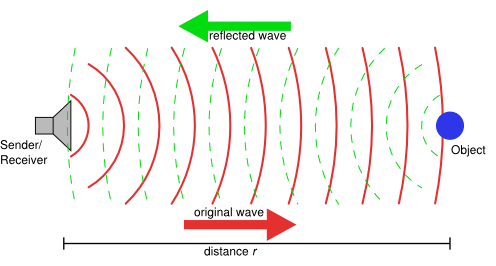
\includegraphics[width=300pt]{img/sonar.png}
    \caption{Sonars in action}
    \label{fig:sonar}
  \end{center}
\end{figure}


The received signal is commonly processed by measuring the time of flight.
This time is depending on the speed of the sound in air, and thus the
temperature, humidity, air pressure, and so on may effect measurements.
\\
The knowledge of time of flight enables the computation of the distance
to the target, which reflected the pulse.
\\
The sonar field of view is a cone and the sensitive area increases proportionately
with the distance. It is necessary to introduce an inhibition time to avoid the false
obstacles due to the ping signal. On the other hand, the inhibition time does
not allow reading distance too short.
\\
The main drawback with the sonar sensor is its wide beam of perception, which
causes the fact that it is impossible from reading returned data to identify
the object position within the beam. Some of the other sonar drawback are specular
reflection; the possibility of a crosstalk when using multiple sensors
or multiple robot.
\\
Nevertheless, the sonar is the sensor most commonly used in robotics, because
widely available, cheap, and easy to controller.

\subsubsection{Bumper}
\label{sec:mobile:bumper}


\subsubsection{Vision}
\label{sec:mobile:vision}


\subsubsection{Odometry}
\label{sec:mobile:odometry}

\subsubsection{Inertial}
\label{sec:mobile:inertial}

\subsubsection{Magnetic compass}
\label{sec:mobile:compass}

\subsubsection{Video based positioning}
\label{sec:mobile:video}

